\documentclass[12pt,a4paper]{article}
\usepackage[utf8]{inputenc}
\usepackage[brazil]{babel}
\usepackage{graphicx} \graphicspath{ {../img/} }
\usepackage{hyperref}
\usepackage{abnt-alf}
\usepackage[top=3cm,bottom=2cm,left=3cm,right=2cm]{geometry}
\usepackage{indentfirst}
\usepackage[table,xcdraw]{xcolor}
\usepackage{subfigure}
\usepackage{amsmath}
\usepackage{import}

% Criar nova pagina a cada nova section
\let\stdsection\section
\renewcommand\section{\newpage\stdsection}

\begin{document}

\citeoption{abnt-etal-cite=3}
\citeoption{abnt-etal-list=5}
\citeoption{abnt-etal-text=3}

% CAPA
\pagestyle{empty}
\begin{center}
\large  \textbf{UNIVERSIDADE PRESBITERIANA MACKENZIE}
\large  \textbf{PROGRAMA DE PÓS-GRADUAÇÃO EM}\\
\large  \textbf{ENGENHARIA ELÉTRICA}\\
\vskip 2.0cm
\textbf{\large Zorandir Soares Junior}\\
\vskip 4.0cm
\setlength{\baselineskip}{1.5\baselineskip}
\textbf{\large Aperfeiçoando a Representação de Autômatos Celulares Através de \textit{Templates}}\\
\vskip 3.5cm
\end{center}
\vskip 7.3cm
\textbf{\normalsize Orientador: Prof. Dr. Pedro Paulo Balbi de Oliveira }\\
\vskip 1.0cm
\begin{center}
São Paulo\\
\the\year\\
\end{center}
\pagenumbering{roman}
\newpage

% CAPA
\pagestyle{empty}
\begin{center}
\large  \textbf{UNIVERSIDADE PRESBITERIANA MACKENZIE}
\large  \textbf{PROGRAMA DE PÓS-GRADUAÇÃO EM}\\
\large  \textbf{ENGENHARIA ELÉTRICA}\\
\vskip 2.0cm
\textbf{\large Zorandir Soares Junior}\\
\vskip 4.0cm
\setlength{\baselineskip}{1.5\baselineskip}
\textbf{\large Aperfeiçoando a Representação de Autômatos Celulares Através de \textit{Templates}}\\
\vskip 3.5cm
\end{center}
\hfill{\vbox{\hsize=8.5cm\noindent\strut
Documento de qualificação apresentado ao \break
Programa de Pós-Graduação em Engenharia\break
Elétrica da Universidade Presbiteriana\break
Mackenzie como requisito parcial para a\break
obtenção do título de Mestre em Engenharia\break
Elétrica.\break}\\
\strut}
\vskip 3.0cm
\textbf{\normalsize Orientador: Prof. Dr. Pedro Paulo Balbi de Oliveira }\\
\vskip 1.0cm
\begin{center}
São Paulo\\
\the\year\\
\end{center}
\newpage

% RESUMO
\newpage
\thispagestyle{plain}
%\pagenumbering{roman}
\begin{center}
\large  
\textbf{RESUMO}
\end{center}
%\renewcommand{\baselinestretch}{0.6666666}
Templates são representações formais para conjuntos de autômatos celulares (ACs) feitas por meio da generalização das tabelas de transição clássicas. Já existem algoritmos que geram templates para propriedades estáticas e algoritmos que realizam operações como intersecção entre templates e expansão de template. Este projeto de pesquisa introduz a operação de complemento de templates e o funcionamento do algoritmo dessa operação implementada na biblioteca \textit{CATemplates}. Também são apresentados exemplos das possibilidades de uso do templates no problema de paridade, com o apoio das operações de complemento e das operações geradoras de templates de ACs conservativos de paridade e ACs conservativos de estado.
\\[0.5cm]
\begin{flushleft}
{\bf Palavras-chave:} {\it Autômatos celulares, templates, conservabilidade, problema de paridade.}
\end{flushleft}

% ABSTRACT
\newpage
\thispagestyle{plain}
%\pagenumbering{roman}
\begin{center}
\large  
\textbf{ABSTRACT}
\end{center}
%\renewcommand{\baselinestretch}{0.6666666}
Templates are formal representation for cellular automaton sets (CAs) made through the generalization of the classical transitions table. Already there are algorithms that generate templates for static properties and algorithms that perform operations such as intersection between templates and template expansion. In this research project it is introduced the templates complement operating and explained the functioning of the algorithm of this operation implemented in the \textit{CATemplates} package. Also show examples of possibilities of using templates in the parity problem, with the support of complement operations and generating operations of CAs conservative parity and ACs state conservative.
\\[0.5cm]
\begin{flushleft}
{\bf Keywords:} {\it Cellular automaton, templates, conservation, parity problem.}
\end{flushleft}

% SUMÁRIO
\newpage
\thispagestyle{empty}
\tableofcontents

% DESENVOLVIMENTO
\newpage
\pagestyle{plain}
\pagenumbering{arabic}
\renewcommand{\baselinestretch}{1.4} 
\normalsize
\section{INTRODUÇÃO}\label{sec:introducao}
Autômatos Celulares (ACs) são sistemas dinâmicos discretos em tempo e espaço cuja dinâmica tem sido extensivamente estudada e aplicada em diversas áreas. ACs tem a capacidade de, através de regras de comportamentos locais simples, gerar comportamentos globais complexos. De acordo com \citeonline{wolfram1994cellular}, ACs podem também ser considerados uma idealização discreta de equações parciais diferenciais, muitas vezes utilizadas para descrever sistemas naturais.

Existem diversas famílias de autômatos celulares estudadas. Devido ao rápido crescimento das famílias dos ACs, de acordo com a variação dos parâmetros de raio e estado, uma das famílias mais estudadas é a do espaço elementar por possuir apenas 256 regras.

Há casos em que os estudos de ACs concentram-se em algum comportamento obtido através de restrições aplicadas às tabelas de transição. Os ACs confinados, criados por \citeonline{theyssier2004captive}, são um dos casos que se pode usar como exemplo. Esses comportamentos e propriedades obtidos através de restrições aplicadas à tabela de transições podem ser denominados como propriedades estáticas.

%TODO: Referencia propriedades estáticas
Propriedades estáticas permitem prever determinados comportamentos de um AC sem consultar sua evolução espaço temporal, ou seja, dispensando a simulação do sistema. Propriedades estáticas também podem ser descritas como indicadores de comportamento de uma determinada família de ACs. Um exemplo de propriedade estática, descrita posteriormente em mais detalhes, é a conservabilidade de paridade. A conservabilidade de paridade define um tipo de AC binário que mantêm o número de estados com valor $1$ sempre com a mesma paridade.

Existem algumas formas de representar propriedades estáticas, e essa representação é crucial pois culmina na eliminação da necessidade de se buscar uma propriedade analisando todo o espaço de um AC. Os autores \citeonline{li1990structure} introduziram variáveis na representação de conjuntos de tabelas de transição. Por meio de grafos de De Bruijn, os autores Betel, De Oliveira e Flocchini (\citeyear{Betel2013}) representam um conjunto de ACs na busca pela solução do problema de paridade. Mais recentemente foi estabelecida uma representação formal para conjuntos de ACs denominada \textit{Templates} \cite{deOliveira2014,deOliveira2014b}. Para se trabalhar com  \textit{Templates} foi criada a biblioteca \textit{CATemplates} \cite{CATemplates}, desenvolvida na linguagem do software \textit{Wolfram Mathematica} \cite{woframMathematica10}.

Templates tem a capacidade de representar conjuntos de ACs sem a necessidade de se operar uma busca em todo espaço original do AC. Essa capacidade dos templates é o principal motivador deste trabalho, visto que essa habilidade é muito importante para a resolução de diversos problemas que buscam por regras com algum comportamento específico.

\subsection{Objetivos}
Este projeto de pesquisa tem como objetivo principal o desenvolvimento de novos algoritmos para geração de templates baseado em propriedades estáticas, bem como apresentar o funcionamento da operação de complemento de templates. Ademais esse projeto propõe-se a apresentar exemplos da utilidade de templates em problemas típicos de autômatos celulares, como o problema de paridade e o problema de densidade.

Até o presente momento os seguintes itens já foram concluídos:
      \begin{itemize}
          \item Implementação da operação de complemento de templates em autômatos celulares binários.
          \item Apresentação de um conjunto de processos que restringem o espaço de busca para a solução do problema de paridade, exemplificando a utilidade de templates em problemas típicos de autômatos celulares.
      \end{itemize}

\subsection{Organização do Documento}
Este documento está organizado da seguinte forma: na Seção \ref{sec:acs} são detalhados os ACs, assim como alguma de suas propriedades. A Seção \ref{sec:templates} apresenta em mais detalhes o funcionamento dos templates, assim como descreve o funcionamentos de duas de suas principais operações. A Seção \ref{sec:propriedadesEstaticas} apresenta algumas propriedade estáticas e explica o funcionamento de suas respectivas operações de geração de template. A Seção \ref{sec:aplicacao} apresenta os resultados parciais desse projeto de pesquisa. Por fim, a Seção \ref{sec:conclusao} apresenta as considerações finais do presente trabalho.








\section{AUTÔMATOS CELULARES}\label{sec:acs}
Autômatos celulares são idealizações matemáticas simples dos sistemas naturais. Eles consistem em um reticulado de campos discretos usualmente idênticos, onde cada campo pode assumir um conjunto finitos de, geralmente, valores inteiros. Os valores dos campos evoluem em tempo discreto de acordo com regras determinísticas que especificam o valor de cada campo de acordo com os campos das vizinhanças \cite{wolfram1994cellular}.

Uma definição parecida é dada por \citeonline{weisstein2015}, que define um AC como um conjunto de células ``coloridas'' em um reticulado com forma previamente especificada que evolui ao longo de uma série de passos de tempo discreto, de acordo com um conjunto de regras baseadas nos estados de células vizinhas. As regras são aplicadas de forma iterativa para o número de passos de tempo desejado.

Os autômatos celulares são compostos por células distribuídas em um reticulado. Essas células mudam de estado ao longo de passos de tempo e de acordo com regras locais. O conjunto de células em determinado passo de tempo é denominado configuração ou estado global e são as configurações que descrevem a evolução espaço temporal de um AC. 

Autômatos celulares podem operar com reticulados em qualquer número de dimensões. Os primeiros ACs eram bidimensionais e foram criados por \citeonline{neumann1966theory} para serem usados como um modelo formal de auto reprodução de sistemas biológicos. Outro conhecido AC bidimensional é o ``Jogo da Vida'' (ou ``Game of Life''), esse AC, criado por John Conway, fez sua primeira aparição em uma coluna de jogos matemáticos \cite{GardnerM1970}. Entre os AC unidimensionais, os mais conhecidos são os do espaço elementar, que foram sistematicamente estudados por \citeonline{wolfram1983statistical}.

Independente da dimensionalidade do reticulado, é necessário definir como o AC se comportará nas bordas. Um tratamento típico é a aplicação da condição de contorno periódica nas extremidades. Ou seja, tratar reticulados unidimensionais como um anel, e bidimensionais como toro (ou toroide). Esses tratamentos podem ser visualizados na Figura \ref{fig:anel} e na Figura \ref{fig:toro}, respectivamente.  
	\begin{figure}[h!]
	  \centering
	  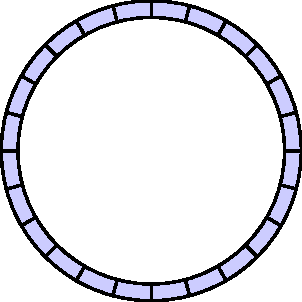
\includegraphics[width=.3\textwidth]{fig_circularList.pdf}
	  \caption{Condição de contorno periódica em um reticulado unidimensional formando um anel.}
	  \label{fig:anel}
	\end{figure}

	\begin{figure}[h!]
	  \centering
  	  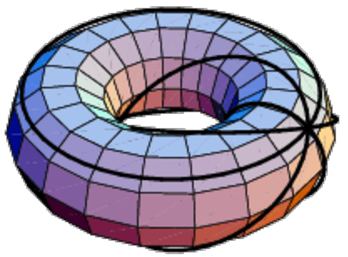
\includegraphics{fig_toro.pdf}
	  \caption{Condição de contorno periódica em um reticulado bidimensional formando um toroide.}
	  \label{fig:toro}
	\end{figure}


%Estados; regras locais; e raio
As células de um autômato celular podem apresentar $k$ estados. O valor desses estados é representado ou por cores ou por valores inteiros no intervalo $[0, k-1]$. O estado de uma célula pode ser modificado pelas funções locais, que são o conjunto de regras que determinam o novo valor de uma célula baseado em seu estado atual e nos estados das células adjacentes. Para que as funções locais atualizem os valores de uma célula, é necessário que um raio $r$ seja definido. Esse raio $r$ representa o número de células adjacentes que serão analisadas em cada direção pelas funções locais.

%vizinhanças
Além do raio, é preciso determinar o formato de vizinhança que será utilizada nos parâmetros da função local. Duas vizinhanças bem comuns em ACs bidimensionais são as vizinhanças de von Neumann \cite{weisstein2015b} e Moore \cite{weisstein2015c}. Na Figura \ref{fig:vVonNeumann} e na Figura \ref{fig:vMoore} são apresentadas, para raios de 0 a 3, as vizinhanças de von Neumann e Moore, respectivamente. No caso dos ACs unidimensionais, as vizinhanças são definidas apenas pelo raio $r$ e ele descreve quantas células a esquerda e direita da célula atual serão consideras pela função local.

	\begin{figure}[h!]
	  \centering
	  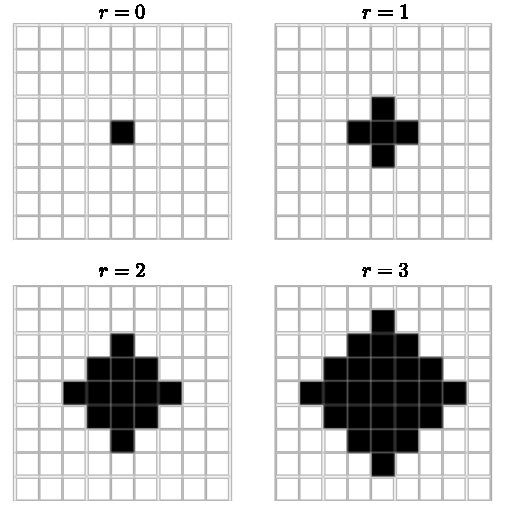
\includegraphics[width=0.45\textwidth]{fig_vVonNeumann.pdf}
	  \caption{Vizinhança de von Neumann com raio $r$ igual a 0, 1, 2 e 3. Essa foi a vizinhança utilizada nos primeiros trabalhos de von Neumann \cite{weisstein2015b}.}
	  \label{fig:vVonNeumann}
	\end{figure}

	\begin{figure}[h!]
	  \centering
  	  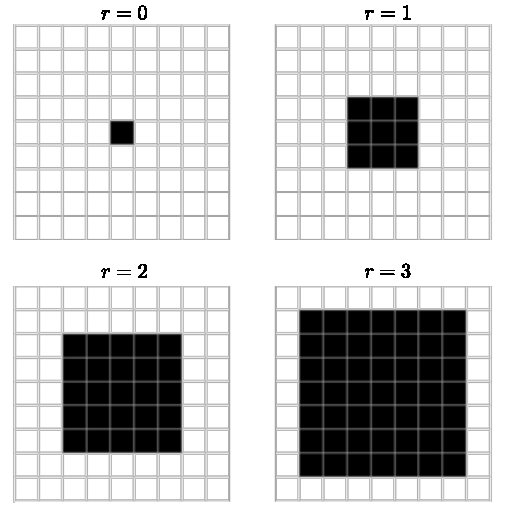
\includegraphics[width=0.45\textwidth]{fig_vMoore.pdf}
	  \caption{Vizinhança de Moore com raio $r$ igual a 0, 1, 2 e 3. Essa foi a vizinhança utilizada no jogo da vida \cite{weisstein2015c}.}
	  \label{fig:vMoore}
	\end{figure}

%Famílias de autômatos Celulares; e Autômatos Celulares Elementares.
Uma família de autômatos celulares é definida pelo raio, número de estados, tipo de vizinhança e a dimensionalidade das configurações. Autômatos celulares unidimensionais de raio $r=1$ e $k=2$ são conhecidos como a família dos autômatos celulares elementares.

Todo AC é regido por um conjunto de regras locais que determinam como ficarão as configurações no próximo passo de tempo de acordo com as configurações de vizinhança recebidas. Existem diversas maneiras de representar essas regras locais, a mais comum são as tabelas de transições. A tabela de transições é uma $n-$upla em que os elementos são todos os possíveis estados de vizinhanças de uma célula acrescentados de um estado que representa a transição que ocorrerá. A Equação \ref{eq:nupla} representa a $n$-upla da regra 30.
\begin{equation}
\begin{split}
(((1,1,1),0),((1,1,0),0),((1,0,1),0),((1,0,0),1),\\
((0,1,1),1),((0,1,0),1),((0,0,1),1),((0,0,0),0))
\label{eq:nupla}
\end{split}
\end{equation}

Uma outra forma de representar uma tabela de transições é a forma icônica. Na forma icônica o bit $1$ é representado por um ícone na cor preta, e o bit $0$ por um ícone na cor branca. Cada uma das transições de estados é representada por um conjunto de ícones que representa a vizinhança na parte superior, e um ícone para representar o estado resultante após a transição na parte inferior. A Figura \ref{fig:repIconicaR30} mostra a representação icônica da regra 30.

	\begin{figure}[h!]
	  \centering
	  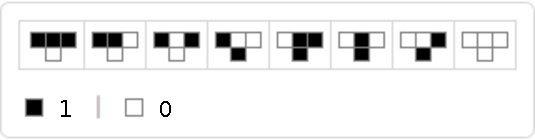
\includegraphics[width=0.6\textwidth]{fig_repIconicaR30.pdf}
	  \caption{Representação icônica da regra 30.}
	  \label{fig:repIconicaR30}
	\end{figure}

Além dessas formas de representação, ainda existe a forma $k$-aria em que, sabendo-se o valor atribuído para $k$ e $r$, elimina-se a representação das vizinhanças e deixa-se apenas as representações resultantes. Na Equação \ref{eq:karia} é possível ver a representação $k$-aria da regra 30. O número da regra é obtido ao se converter a representação $k$-aria para decimal. Esse número é um identificador único em família de autômatos celulares, ou seja, sempre representa apenas uma tabela de transições de estado.
\begin{equation}
(0,0,0,1,1,1,1,0)
\label{eq:karia}
\end{equation}

O número de regras de um espaço é definido pela Equação \ref{eq:tamFamilia}:
\begin{equation}
k^{k^{2r+1}}
\label{eq:tamFamilia}
\end{equation}

No espaço elementar há $2^{2^{3}} = 256$ regras. Aumentando o raio $r=2$, obtemos uma família de $2^{2^{5}} = 4.294.967.296$ regras. Para $k=3$ e $r=1$, obtém-se um espaço de ACs com $3^{3^{3}} = 7.625.597.484.987$ regras. Logo, é fácil perceber que qualquer modificação nas variáveis $k$ e $r$ geram famílias com número de regras muito grande. Famílias grandes de ACs representam um desafio na hora de encontrar ACs com propriedades específicas, já que procurar regras através de força bruta em um espaço muito grande se torna uma tarefa extremamente improdutiva.

Para contornar esse problema, é comum utilizar algumas propriedades estáticas para restringir as regras do espaço no qual serão feitas as buscas. Alguns exemplos de propriedades estáticas que podem auxiliar nesse ``filtro'' são o confinamento, conservabilidade de estados e conservabilidade de paridade. Todas as propriedades estáticas citadas anteriormente são detalhadas na Seção \ref{sec:propriedadesEstaticas}.

O problema da paridade é um dos problemas que envolvem fazer a ligação entre comportamento local e comportamento global de um autômato celular. Para o problema de paridade, nesse projeto, considera-se um AC binário, unidimensional e com condição de contorno periódica. Se uma configuração inicial contiver um número ímpar de estados com valor 1, o AC deve convergir para que todas as células estejam preenchidas com 1, caso contrário, ele deve convergir para todos os estados com o valor 0. Por conta da própria definição do problema, fica simples perceber que essas condições não podem ser satisfeitas em uma grelha de tamanho par, afinal uma configuração com todos os estados apresentando o mesmo valor não poderia ser um estado quiescente. Devido essa questão, pode-se dizer que as regras que solucionam o problema de paridade em ACs são \textit{perfeitas} se eles resolverem o problema de paridade em qualquer configuração inicial arbitrária para ACs de tamanho ímpar \cite{Betel2013}. Ainda em relação ao problema de paridade, Betel, De Oliveira e Flocchini (\citeyear{Betel2013}) descrevem duas propriedades básicas: se $f$ é a regra local que resolve o problema de paridade, então $f(0, \dots, 0) = 0$ e $f(1, \dots, 1) = 1$. A segunda propriedade define que para uma regra preservar a configuração de paridade ela deve apresentar número par de transições ativas. Em outras palavras, toda aplicação da regra deve levar a uma nova configuração com a mesma paridade.

Procurar uma regra que resolva o problema de paridade em autômatos celulares unidimensionais de raio 3, por exemplo, por meio de buscas por força bruta acarretaria em testar mais de 340 undecilhões de regras. Uma maneira de facilitar essa busca é restringir as regras através propriedades estáticas, mas é necessário uma forma de representar essas propriedades e até mesmo aplicar operações como intersecção e complemento entre elas. Nesse ponto que os \textit{templates} apresentam-se de uma forma interessante e útil para representar conjuntos de regras com determinada propriedade. Templates de ACs são uma generalizações das tabelas de transições que permitem representar espaços inteiros de ACs \cite{Verardo2014}.








\section{TEMPLATES}\label{sec:templates}
\textit{Templates} de autômatos celulares são uma generalização de tabelas de transições que faz com que um templates seja capaz de representar famílias de autômatos celulares. Os templates foram criados por De Oliveira e Verardo (\citeyear{deOliveira2014}) e implementada como um algoritmo na linguagem do software \textit{Wolfram Mathematica} \cite{woframMathematica10}, atualmente disponíveis na biblioteca \textit{open source CATemplates} \cite{CATemplates} no GitHub.

Formalmente, um \textit{template} é uma $n$-upla formada por $k^{2r+1}$ itens, e cada item $i$ representa uma função $g_i(x_0,x_1,\dots,x_{k^{2r+1}-1})$. As variáveis $x_i$ podem assumir qualquer estado entre 0 e $k-1$, logo no caso binário $x_i$ pode assumir os valores 0 e 1. É possível limitar os valores possíveis de $x_i$ através da notação $x_i \in C$, onde $C$ é um conjunto representando os possíveis valores de $x_i$. Entretanto vale frisar que no caso binário não tem lógica implementar uma notação como $x_i \in {1}$ ou $x_i \in {0}$ pois os templates também aceitam constante, sendo essas notações equivalente à apenas as constante $1$ e $0$, respectivamente.

Exemplificando, dado um template $T_1 = (1,1,1,1,1-x_1,x_2,x_1,0)$, ele representará todas as regras que tenham em sua primeira posição (sempre da direita pra esquerda) o estado 0, nas posições 5, 6, 7 e 8 o estado 1, nas posições 2 e 3 qualquer estado no intervalo $[0,k-1]$ e na posição 4 o estado complementar ao valor de $x_1$. Perceba que o tamanho da $n$-tupla é determinado pela função $k^{2r+1}$, logo no template $T_1$ os únicos valores inteiros possíveis para $k$ e $r$ são 2 e 1 respectivamente. Portanto $T_1$ representará um subespaço dos ACs elementares.

Deste modo o template $T_1$ representam o conjunto de autômatos celulares elementares $\{(1,1,1,1,1,0,0,0),(1,1,1,1,0,0,1,0),(1,1,1,1,1,1,0,0),(1,1,1,1,0,1,1,0)\}$, ou em sua forma decimal $\{248,242,252,246\}$.

Cada template tem um número de substituições máximo igual a $k^m$, sendo o $m$ o número de variáveis livres. O maior template possível de uma família de ACs é o \textit{template base}, em que todas as variáveis são livres. O menor é o \textit{template constante}, em que não há variáveis livres, logo representa apenas uma regra. As $8$-uplas representada pela Equação \ref{eq:templateConstante} representa um template constante que pode ser associado apenas a regra 30. 
\begin{equation}
(0,0,0,1,1,1,1,0)
\label{eq:templateConstante}
\end{equation}

Já a $8$-uplas, apresentada na Equação \ref{eq:templateBase}, representa um template base que está associado a todas as 256 regras do espaço elementar já que, para $m = 8$, temos $2^m = 256 $.
\begin{equation}
(x_7,x_6,x_5,x_4,x_3,x_2,x_1,x_0)
\label{eq:templateBase}
\end{equation}

É importante enfatizar que nem sempre o número de substituições é igual a $k^m$. Isto ocorre pois algumas substituições podem originar tabelas de transições inválidas. O template $(1,1,1,1,1,x_0+x_1,x_1,x_0)$, por exemplo, não pode apresentar as substituições $x_0=1$ e $x_1=1$ ao mesmo tempo, pois isso faz com que $x_0 + x_1 \notin [0, k-1]$, invalidando assim essa substituição.

A representação de famílias de autômatos celulares através de templates, possibilita a utilização de templates para problemas já bem conhecidos da área de ACs. Um exemplo de problema que pode se beneficiar dos templates é o problema da paridade.

A Figura \ref{fig:parity-rule} ilustra o desenvolvimento espaço temporal de uma regra que usualmente resolve o problema de paridade. Nessa imagem o desenvolvimento temporal à esquerda contém, em sua configuração inicial, um número par de estados igual a 1, já na evolução temporal ilustrada à direita há um número ímpar de estados igual a 1.

\begin{figure}[h!]
	\center
	\subfigure[CI com número ímpar de 1s]{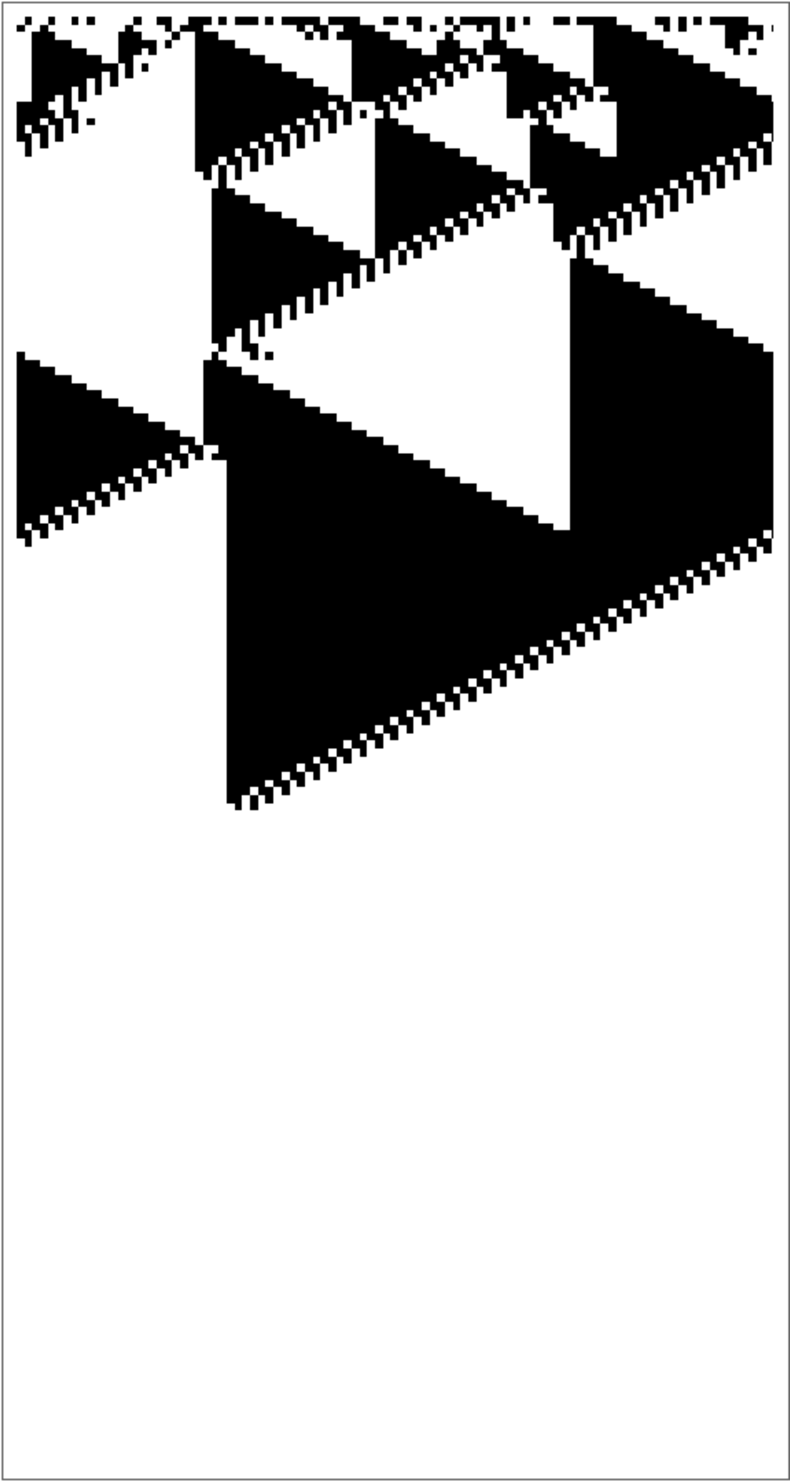
\includegraphics[width=4.8cm]{regra-1-par.pdf}}
	\qquad
	\subfigure[CI com número par de 1s]{
\includegraphics[width=4.8cm]{regra-1-impar.pdf}}
	\caption{Desenvolvimento espaço temporal de um AC que usualmente resolve o problema de paridade.}
	\label{fig:parity-rule}
\end{figure}

O estudo do problema de paridade é interessante pois ajuda a compreender um problema ainda sem solução em ACs, que é, que a despeito da habilidade de realizar computações, pouco se sabe sobre como se deve projetar transições de estado locais que levem a um comportamento global pré-determinado. Entretanto, entender o impacto das interações locais nas soluções globais influi em diversos sistemas de computação emergente. Entender a influência que o tamanho da vizinhança dos autômatos celulares apresenta na computabilidade pode apresentar consequências úteis para o projeto de ACs e para a compreensão de sistemas emergentes complexos em geral.

Estudos feitos sobre o problema de paridade já levaram ao conhecimento de que o problema não tem solução perfeita para ACs elementares e de raio 2, todavia já foi descoberta uma regra perfeita que soluciona o problema de paridade para raio 4. Em relação aos ACs de raio 3, ainda não foi encontrada solução perfeita e há evidências empíricas desfavoráveis a uma solução para esse raio \cite{Betel2013}.

Betel, De Oliveira e Flocchini (\citeyear{Betel2013}), buscando definir se o problema de paridade em ACs de raio 2 apresenta alguma solução perfeita, encontraram de forma analítica como as transações de estado de supostas regras que resolvessem o problema de paridade deveriam ser. Com isso, utilizando grafos de \textit{De Bruijn} foram definidas quais variáveis deveriam ser estáticas, quais deveriam ser livres e quais deveriam apresentar interdependência. Com essas definições foram definidas duas famílias de ACs. Os grafos ilustrados na Figura \ref{fig:grafosDeBruijn} e na Figura \ref{fig:grafosDeBruijn2} são os grafos desenvolvidos por Betel, De Oliveira e Flocchini (\citeyear{Betel2013}).

\begin{figure}[h!]
  \centering
  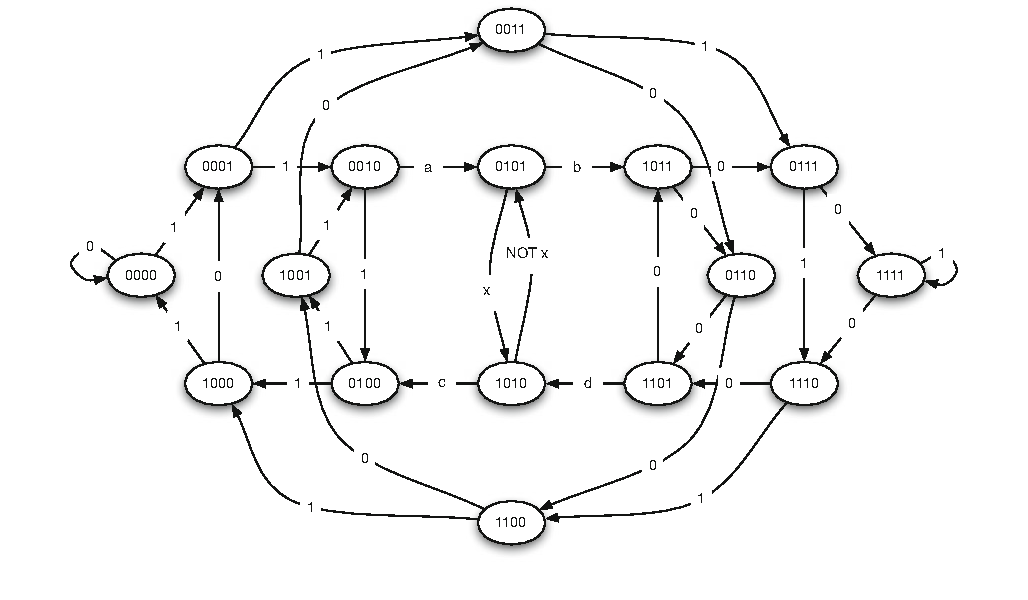
\includegraphics[width=.8\textwidth]{grafo1.pdf}
    \caption{Grafo de De Bruijn representando regras que possivelmente solucionem o problema de paridade.}
    \label{fig:grafosDeBruijn}
\end{figure}

Ambos os grafos apresentam as variáveis livres $a, b, c, d \text{ e } x$ e uma interdependência, em que uma transição de estado deve ter o valor oposto à variável $x$. A única diferença entre os dois grafos está nas variáveis estáticas.

\begin{figure}[h!]
  \centering
  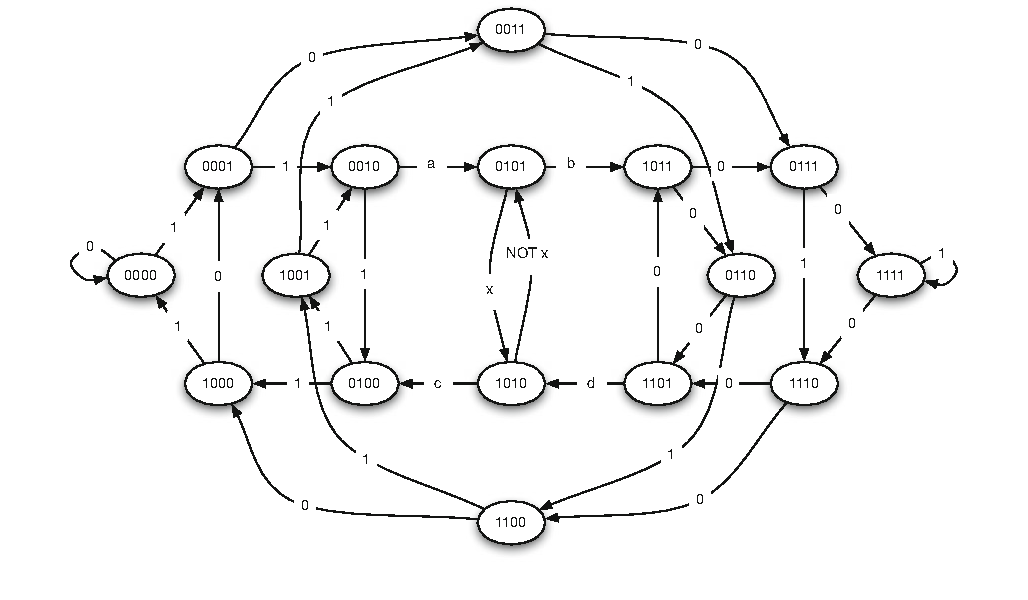
\includegraphics[width=1\textwidth]{grafo2.pdf}
    \caption{Outro grafo de De Bruijn representando regras que possivelmente solucionem o problema de paridade.}
    \label{fig:grafosDeBruijn2}
\end{figure}

Ao utilizar os grafos de \textit{De Bruijn} fixando algumas transições de estado a família de ACs em que se procurava as regras que solucionavam o problema de paridade foi restringida para apenas 64 regras. Ao se restringir o espaço de busca, antes composto por $2^{32}$ regras, as regras puderam ser estudadas em mais detalhes até que falhassem. Entretanto, conforme mostrado em \cite{Verardo2014}, a representação desse espaço de 64 regras pode ser equivalentemente representado por meio de \textit{templates}. O template \ref{eq:templateParidade1} representa o mesmo espaço que a Figura \ref{fig:grafosDeBruijn}, já o template \ref{eq:templateParidade2} é equivalente a Figura \ref{fig:grafosDeBruijn2}.
\begin{equation}
\left(0,1,1,1,1,x_{26},0,1,1,1,1-x_{10},x_{20},0,0,1,0,1,0,1,0,x_{11},x_{10},0,0,1,0,x_5,0,1,0,0,1\right)
\label{eq:templateParidade1}
\end{equation}
\begin{equation}
\left(0,1,1,0,1,x_{26},1,0,1,1,1-x_{10},x_{20},0,1,1,0,1,0,1,1,x_{11},x_{10},0,0,1,0,x_5,0,0,0,0,1\right)
\label{eq:templateParidade2}
\end{equation}


\newpage\newpage
\subsection{Expansão de Templates}
	Expansão é o processo no qual se obtêm todas as tabelas de transição $R_k$ associadas a um template $T$.
	A operação de expansão foi apresentada por \citeonline{Verardo2014} e foi descrita em mais detalhes da seguinte maneira:

	\begin{equation}
	E(T)=R_k
	\end{equation}

	A operação de expansão pode ser dividida em dois passo, em que o primeiro consiste em efetuar todas as $i$ substituições de variáveis, sendo que $i$ pertence ao intervalo discreto $[0,k^m-1]$. Considere como exemplo o template $T_1 = (1,1,1,1,1-x_1,x_2,x_1,0)$, o primeiro passo do processo de expansão consiste em encontrar as tabelas $k$-arias resultantes das combinações possíveis das substituições de $x_1$ e $x_2$, conforme pode ser melhor visualizado na Tabela \ref{tab:expansionProcess}.

	\begin{table}[h!]
	\centering
	\caption{Processo de expansão}
	{
		\vspace{0.3cm}
		\begin{tabular}{cccc}
		\hline
		$i$ & $x_2$ & $x_1$ & tabela $k$-aria resultante \\
		\hline
		0	&	0	&	0	&	(1,1,1,1,1,0,0,0)	\\
		1	&	0	&	1	&	(1,1,1,1,1,1,0,0)	\\
		2	&	1	&	0	&	(1,1,1,1,0,0,1,0)	\\
		3	&	1	&	1	&	(1,1,1,1,0,1,1,0)	\\
		\hline
		\end{tabular}
	}
	\label{tab:expansionProcess}
	\end{table}

	O segundo passo da operação de expansão é eliminar as tabelas $k$-aria inválidas. No caso do template $T_1$ todas as tabelas resultantes eram válidas, mas nem sempre isso ocorre. No template $T_2 = (1,1,1,1,1,x_0+x_1,x_1,x_0)$, por exemplo, a substituição $x_0 = 1$ e $x_1 = 1$ resulta numa tabela $k$-aria inválida pois a terceira posição apresenta um estado com um valor fora do interval $[0,k-1]$, para $k=2$. A Tabela \ref{tab:invalideExpansion} evidência melhor essa substituição inválida.

	\begin{table}[h!]
	\centering
	\caption{Processo de expansão}
	{
		\vspace{0.3cm}
		\begin{tabular}{cccc}
		\hline
		$i$ & $x_1$ & $x_0$ & tabela $k$-aria resultante \\
		\hline
		0	&	0	&	0	&	(1,1,1,1,1,0,0,0)	\\
		1	&	0	&	1	&	(1,1,1,1,1,1,0,1)	\\
		2	&	1	&	0	&	(1,1,1,1,1,1,1,0)	\\
		3	&	1	&	1	&	(1,1,1,1,1,2,1,1)	\\
		\hline
		\end{tabular}
	}
	\label{tab:invalideExpansion}
	\end{table}

	Ainda há outra maneira em que templates resultam em substituições inválidas, sendo uma delas através da utilização da notação restrição por conjuntos. Considere o templates $T_3 = (2,2,2,2,2,2,2,2,x_0\in \{0,1\})$ da família de $k=3$ e $r=0,5$. A substituição obtida para $i = 2$ seria inválida pois nesse caso $x_0 = 2$ e $2 \notin \{0,1\}$. A Tabela \ref{tab:invalideExpansion2} evidencia melhor esse processo.

	\begin{table}[h!]
	\centering
	\caption{Processo de expansão}
	{
		\vspace{0.3cm}
		\begin{tabular}{cccc}
		\hline
		$i$ & $x_0$ & tabela $k$-aria resultante \\
		\hline
		0	&	0	&	(2,2,2,2,2,2,2,2,0)	\\
		1	&	1	&	(2,2,2,2,2,2,2,2,1)	\\
		2	&	2	&	(2,2,2,2,2,2,2,2,2)	\\
		\hline
		\end{tabular}
	}
	\label{tab:invalideExpansion2}
	\end{table}

	A existência de regras inválidas são os responsáveis por templates que representem um conjunto de regras menores que $k^m$. Essa possibilidade é bastante útil para os templates de regras conservativas e regras confinadas.

	O valor de $i$ sempre representa apenas uma substituição possível para as variáveis livres de um templates. Isso ocorre pois $i$ é a representação decimal da conversão $k$-aria das concatenações dos valores das variáveis livres em ordem decrescente. Exemplificando, considere o templates $T_3 = (2,2,2,2,2,2,2,x_1,x_0\in \{0,1\})$ para $k=3$. O valor de $i=5$ será convertido pelo processo de expansão obtendo-se assim o seu equivalente na base ternária $(1,2)$ e então cada um dos dígitos é atribuído a uma variável, resultando assim no conjunto de substituições ${x_0=2,x_1=1}$.

	A forma com que o valor de $i$ representa apenas uma expansão permite possibilidade de se obter a $i$-ésima expansão de um template. Essa propriedade é relevante devido ao fato da expansão ser uma operação potencialmente custosa, e a possibilidade de ser realizar a $i$-ésima expansão de um template facilita e permite o paralelismo.

\newpage\newpage
\subsection{Intersecção de Templates}
	Intersecção é o processo no qual se obtêm um template que represente o conjunto $R_k$. O conjunto $R_k$ representa todas as regras pertencentes aos dois templates recebidos como parâmetro. É necessário que os dois templates recebidos como parâmetro pertençam ao mesmo espaço. A operação de intersecção foi descrita por \citeonline{Verardo2014} e mostrada em mais detalhes da seguinte maneira:

	\begin{equation}
	I(T_1,T_2)=T_3 \Leftrightarrow E(T_3) = E(T_1) \cap E(T_2)
	\end{equation}

	A operação de intersecção, assim como a de expansão, também é efetuada em duas etapas. Na primeira etapa iguala-se os dois templates e assim obtêm-se um sistema de equações. Esse sistema de equações é então passado como argumento para a função Solve, função essa nativa da \textit{Wolfram Language} \cite{woframMathematica10}. A função Solve retorna então os relacionamentos entre as variáveis, que ao serem aplicados aos templates recebidos, retorna dois template equivalente, bastando escolher um que será o template de intersecção. No caso dos templates não apresentarem intersecção, a função Solve não retornará solução.

	Para melhor compreensão, considere os templates $T_1 = (x_7,x_3,1-x_4,x_4,x_3,x_2,2,x_0)$ e $T_2 = (x_7,1,x_5,0,x_3,x_2,2,2)$, ambos com $r=0.5$ e $k=3$. Esse templates serão transformado em um sistema de equações como demonstrado na Equação \ref{eq:interseccao}.

	\begin{equation}
	\left\{\begin{matrix}
	x_7   & = & x_7 \\ 
	x_3   & = & 1 \\ 
	1-x_4 & = & x_5    \\ 
	x_4   & = & 0    \\ 
	x_3   & = & x_3    \\ 
	x_2   & = & x_2   \\ 
	2     & = & 2   \\ 
	x_0   & = & 2
	\end{matrix}\right.
	\label{eq:interseccao}
	\end{equation}

	Esse sistema de equações é passado então como argumento para a função Solve, que por sua vez retorna um conjunto solução $S$, que nesse exemplo é $S = \{x_0 = 2, x_3 = 1, x_4 = 0, x_5 = 1 - x_4, x_6 = 0\}$. O conjunto $S$ é aplicado como um conjunto de substituições sobre os dois templates recebidos como parâmetro, que em caso de templates sem restrição de variáveis sempre retorna o mesmo template. Neste exemplo, após aplicada as substituições do conjunto de soluções $S$, obtêm-se como resultado o template $T_3 = (x_7, 1, 1, 0, 1, x_2, 2, 2)$.

	A segunda etapa do algoritmo apenas é aplicada para templates com alguma restrição de variável. Essa etapa consiste em extrair as expressões que estabelecem as restrições, e através delas obter um segundo sistema de equações. A solução desse sistema ou pode ser vazia, expressando assim que os templates não tem intersecção, ou pode indicar os valores que as variáveis com restrição podem assumir.

	Para exemplificar essa segunda etapa, considere os templates $T_{r1} = (x_7 \in \{0,1,2\},x_3,1-x_4,x_4,x_3,x_2 \in \{1,2\},2,x_0)$ e $T_{r2} = (x_7 \in \{0,1\},1,x_5,0,x_3,x_2 \in \{1\},2,2)$. A primeira etapa ocorre normalmente, entretanto, quando as substituições do conjunto $S$ forem aplicadas nos templates recebidos, não será mais obtido templates iguais. Nesse caso o conjunto de templates obtidos será $\{(x_7 \in \{0,1,2\}, 1, 1, 0, 1, x_2 \in \{1,2\}, 2, 2), (x_7 \in \{0,1\}, 1, 1, 0, 1, x_2 \in \{1\}, 2, 2)\}$. Na sequencia o algoritmos faz a extração das expressões de restrição de variáveis e obtêm o conjunto $\{x_7 \in \{0,1\}, x_2 \in \{1,2\}, x_2 \in \{1\} \}$. Esse conjunto é então convertido para o sistema de equações representadas pela Equação \ref{eq:interseccaoRestrita}.

	\begin{equation}
	\left\{\begin{matrix}
	x_7	  = 0 	& \vee &	x_7	=	1 & \vee &	x_7	= 2	\\ 
	x_7   = 0 	& \vee &	x_7	=	1					\\ 
	x_2   = 1 	& \vee &	x_2	=	2					\\ 
	x_2	  =	1											\\ 
	\end{matrix}\right.
	\label{eq:interseccaoRestrita}
	\end{equation}

	Esse sistema de equações é então passado como argumento para a função Solve, que retorna seu conjunto solução. Por fim o algoritmo usa o conjunto solução retornado para remover as restrições da variável $x_2$, transformando-a no valor $1$, e restringi a variável $x_7$ apenas ao conjunto $\{0,1\}$. O template de intersecção gerado por todo esse processo é representado pela Equação \ref{eq:templateIntescecao}.

	\begin{equation}
	T_{r3} = (x_7 \in \{0,1\}, x_3, 1-x_4, x_4, x_3, 1, 2, x_0)
	\label{eq:templateIntescecao}
	\end{equation}

	Vale frisar que o template $T_{r2}$ também poderia ser representado substituindo a variável $x_2$ e seu conjunto de restrição $\{1\}$ apenas pelo valor constante $1$, como mostrado a seguir: $T_{r2} = (x_7 \in \{0,1\}, 1, x_5, 0, x_3, 1, 2, 2)$. Esse tipo de mudança é sempre preterido pois variáveis a mais acarretam em mais processamento.

	No caso binário, ou seja $k = 2$, a notação de restrição nunca é necessária visto que ou a restrição terá apenas um valor factível, sendo preferível que essa variável e sua restrição sejam substituídas por um valor constante, ou a variável poderá assumir qualquer estado sendo assim, por definição, uma variável livre.





\section[REPRESENTAÇÃO DE PROPRIEDADES ESTÁTICAS POR MEIO DE TEMPLATES]{REPRESENTAÇÃO DE PROPRIEDADES \\ ESTÁTICAS POR MEIO DE TEMPLATES}
\label{sec:propriedadesEstaticas}

	Em ACs, propriedades estáticas são propriedades computadas com base nas tabelas de transição. Essas propriedades permitem prever determinados comportamentos de um ACs sem consultar sua evolução espaço temporal. 

	Esta seção descreverá algumas propriedades estáticas e os algoritmos geradores de templates que as representam. Todos algoritmos explicados estão implementados na biblioteca \textit{CATemplates} \cite{CATemplates}.

	\subsection{Conservabilidade de Estados e Conservabilidade de Paridade}
	Conservabilidade de estados é uma propriedade estática que determina que a soma dos estados de um determinado autômato celular não deve se alterar durante a evolução espaço temporal, independente da configuração inicial passada.

	De acordo com Boccara e Fukś (\citeyear{boccara2002}), um AC é conservativo quando cada uma de suas regras locais $f$ de vizinhança $(\alpha_0,\alpha_1, \dots, \alpha_{n-1})$ respeita as condições descritas na Equação \ref{eq:conservativeCA}.

	\begin{equation}
	\begin{split}
	f(\alpha_0,\alpha_1, \dots,\alpha_{n-1}) = \alpha_0 + (\sum_{i=0}^{n-2}f(0_0,0_1, \dots,0_i,\alpha_1,\alpha_2, \dots,\alpha_{n-1}) \\- f(0_0,0_1, \dots,0_i,\alpha_0,\alpha_1, \dots,\alpha_{n-i-1}))
	\label{eq:conservativeCA}
	\end{split}
	\end{equation}

	Para exemplificar, considere a regra 204 do espaço elementar. Por meio da condição mostrada na Equação \ref{eq:conservativeCA}, será provado que essa regra é conservativa, já que satisfaz a condição. A Equação \ref{eq:ruleTable204} representa a tabela de transições da regra 204.

	\begin{equation}
	\begin{split}
	(((1,1,1),1),((1,1,0),1),\\((1,0,1),0),((1,0,0),0),\\((0,1,1),1),((0,1,0),1),\\((0,0,1),0),((0,0,0),0))
	\label{eq:ruleTable204}
	\end{split}
	\end{equation}

	Como demonstra \citeonline{Verardo2014}, a aplicação das condições da Equação \ref{eq:conservativeCA} nas tabelas de transições de ACs do espaço elementar, sempre resultará no sistema descrito pela Equação \ref{eq:conservativeLinearSystem}.

	\begin{equation}
	\left\{\begin{matrix}
	 f(0,0,0) = 0 + (f(0,0,0) - f(0,0,0)) + (f(0,0,0) - f(0,0,0))\\ 
	 f(0,0,1) = 0 + (f(0,0,1) - f(0,0,0)) + (f(0,0,0) - f(0,0,0))\\ 
	 f(0,1,0) = 0 + (f(0,1,0) - f(0,0,1)) + (f(0,0,1) - f(0,0,0))\\ 
	 f(0,1,1) = 0 + (f(0,1,1) - f(0,0,1)) + (f(0,0,1) - f(0,0,0))\\ 
	 f(1,0,0) = 1 + (f(0,0,0) - f(0,1,0)) + (f(0,0,0) - f(0,0,1))\\ 
	 f(1,0,1) = 1 + (f(0,0,1) - f(0,1,0)) + (f(0,0,0) - f(0,0,1))\\ 
	 f(1,1,0) = 1 + (f(0,1,0) - f(0,1,1)) + (f(0,0,1) - f(0,0,1))\\ 
	 f(1,1,1) = 1 + (f(0,1,1) - f(0,1,1)) + (f(0,0,1) - f(0,0,1))
	\end{matrix}\right.
	\label{eq:conservativeLinearSystem}
	\end{equation}

	A Equação \ref{eq:conservativeLinearSystem} simplificada é representada pela Equação \ref{eq:conservativeLinearSystem2}.

	\begin{equation}
	\left\{\begin{matrix}
	 f(0,0,0) & = & 0 		& &\\ 
	 f(0,0,1) & = & f(0,0,1)& & \\ 
	 f(0,1,0) & = & f(0,1,0)& & \\ 
	 f(0,1,1) & = & f(0,1,1)& & \\ 
	 f(1,0,0) & = & 1 - f(0,0,1) - f(0,1,0) \\ 
	 f(1,0,1) & = & 1 - f(0,1,0) \\ 
	 f(1,1,0) & = & 1 + (f(0,1,0) - f(0,1,1))\\ 
	 f(1,1,1) & = & 1 & &
	\end{matrix}\right.
	\label{eq:conservativeLinearSystem2}
	\end{equation}

	Excluindo-se as condições tautológicas do sistema e atribuindo os valores das funções locais $f$ conforme a tabela de transições da regra 204, é obtido o sistema descrito pela Equação \ref{eq:conservativeAC204}. Esse sistema, ao não apresentar condições contraditórias ou falsas, prova que a regra 204 é conservativa.

	\begin{equation}
	\left\{\begin{matrix}
	 0 & = & 0 \\ 
	 0 & = & 1 - 0 - 1 \\ 
	 0 & = & 1 - 1 \\ 
	 1 & = & 1 + (1 - 1)\\ 
	 1 & = & 1 
	\end{matrix}\right.
	\label{eq:conservativeAC204}
	\end{equation}

	O algoritmo que gera templates que representam regras conservativas, criado por De Oliveira e Verardo (\citeyear{deOliveira2014}), primeiramente recebe as variáveis $k$ e $r$ definindo assim a família das regras que serão geradas. Em seguida, cria todas as vizinhanças do espaço com exceção das vizinhanças que geram tautologias. E após esses passos, aplica as condições de Boccara e Fukś (\citeyear{boccara2002}). Para se excluir as vizinhanças que geram tautologias, basta excluir as vizinhanças que começam com 0 mas não sejam compostas apenas por 0 \cite{Schranko2010}.

	Para exemplificar o funcionamento do algoritmo, considere um espaço com $k=2$ e $r=1$. Primeiramente o algoritmo obterá o conjunto das vizinhanças que não geram regras tautológicas, portanto será obtido o conjunto $\{(1,1,1),(1,1,0),(1,0,1),(1,0,0),(0,0,0)\}$. Então é criado o sistema de equações \ref{eq:conservativeLinearSystem3}, baseado nas condições de Boccara e Fukś (\citeyear{boccara2002}).

	\begin{equation}
	\left\{\begin{matrix}
	 x_0 & = & 0\\ 
	 x_4 & = & 1 +2x_0 -x_1 -x_2\\ 
	 x_5 & = & 1 +x_0 -x_2\\
	 x_6 & = & 1 +x_2 -x_3\\ 
	 x_7 & = & 1
	\end{matrix}\right.
	\label{eq:conservativeLinearSystem3}
	\end{equation}

	Por fim o algoritmo utiliza a função Solve do \textit{Wofram Mathematica} para simplificar o sistema e utiliza o conjunto solução retornado pela função Solve como regras de substituições. Essas regras de substituições são aplicadas no template base, gerando assim o template das regras conservativas. O template gerado pode ser observado na Equação \ref{eq:conservativeTemplate}, e sua expansão gera as cinco regras conservativas do espaço elementar, após eliminadas as regras inválidas.

	\begin{equation}
	(1,x_2-x_3+1,1-x_2,-x_1-x_2+1,x_3,x_2,x_1,0)
	\label{eq:conservativeTemplate}
	\end{equation}

	O processo de gerar regras conservativas de paridade é bem parecido. Porém as condições estabelecidas por Boccara e Fukś (\citeyear{boccara2002}) são ligeiramente modificadas em relação a Equação \ref{eq:conservativeCA}, de forma que cada uma das funções locais deve respeitar agora as condições da Equação \ref{eq:parityConservativeCA}.

	\begin{equation}
	\begin{split}
	f(\alpha_0,\alpha_1, \dots,\alpha_{n-1}) \equiv \alpha_0 + (\sum_{i=0}^{n-2}f(0_0,0_1, \dots,0_i,\alpha_1,\alpha_2, \dots,\alpha_{n-1}) \\- f(0_0,0_1, \dots,0_i,\alpha_0,\alpha_1, \dots,\alpha_{n-i-1})) \; (mod 2)  
	\label{eq:parityConservativeCA}
	\end{split}
	\end{equation}

	A biblioteca \textit{CATemplates} já tem implementado o algoritmo gerador de templates de regras conservativas de paridade, e conforme será mostrado posteriormente, esse algoritmo pode ser de suma importância na busca de uma solução para o problema de paridade.





	\subsection{Confinamento}
	Os autômatos celulares confinados, ou \textit{captive} em Inglês, são uma classe de AC que se baseiam em uma caracterização de suas funções locais que não adotem estados definidos em qualquer estrutura externa à vizinhança \cite{theyssier2004captive}. 

	\citeonline{theyssier2004captive} formalmente define que dado a função local $f$ de um AC para a vizinhança $(\alpha_0, \dots, \alpha_{2r})$, sendo o $r$ o raio, um AC é considerado confinado se respeitar a condição descrita na Equação \ref{eq:captiveAC}.

	\begin{equation}
	f((\alpha_0, \dots, \alpha_{2r})) = \beta, \beta \in \{\alpha_0, \dots, \alpha_{2r}\}
	\label{eq:captiveAC}
	\end{equation}

	Essa propriedade pode ser facilmente representada através de templates. Para isto, basta restringir as variáveis a um conjunto de valores presentes na vizinhança correspondente. A biblioteca \textit{open source CATemplates} já apresenta um algoritmo que gera as regras confinadas. Esse algoritmo recebe como parâmetro os argumentos $k$ e $r$. Após isso, gera as vizinhanças do espaço e verifica em cada uma das vizinhanças os estados que elas têm. Caso a vizinhança tenha todos os estados do intervalo $[0, k-1]$ essa posição terá uma variável livre no template. Caso a vizinhança tenha apenas um estado a posição correspondente no template assume um valor fixo. Por fim, caso a vizinhança apresente mais de um estado, mas não todos, a posição correspondente do template apresentará uma variável restritas mediante expressões $x_i \in C$.

	É trivial perceber que qualquer AC binário que tenha as funções locais $f((0_0, 0_1,\dots, 0_{2r})) = 0$ e $f((1_0, 1_,1\dots, 1_{2r})) = 1$ é caracterizado como um AC confinado. A Equação \ref{eq:captiveTemplateACE} representa o template de todas as regras confinadas do espaço elementar e as equações \ref{eq:captiveTemplateR05} representam a família de $k=2$ e $r=0,5$.
	\begin{equation}
	(1,x_6,x_5,x_4,x_3,x_2,x_1,0)
	\label{eq:captiveTemplateACE}
	\end{equation}

	\begin{equation}
	(1,x_2,x_1,0)
	\label{eq:captiveTemplateR05}
	\end{equation}

	Por fim, a Equação \ref{eq:captiveTemplateK3} representa a família dos autômatos celulares confinados de $r=1$ e três estados.

	\begin{equation}
	\begin{split}
	(2, x_{25} \in \{1,2\}, x_{24} \in \{0,2\}, x_{23} \in \{1,2\}, x_{22} \in \{1,2\}, x_{21}, x_{20} \in \{0,2\}, x_{19}, x_{18} \in \{0,2\}, \\
	x_{17} \in \{1,2\}, x_{16} \in \{1,2\}, x_{15}, x_{14} \in \{1,2\},1, x_{12} \in \{0,1\}, x_{11}, x_{10} \in \{0,1\}, x_9 \in \{0,1\}, \\
	x_8 \in \{0,2\}, x_7, x_6 \in \{0,2\}, x_5, x_4 \in \{0,1\}, x_3 \in \{0,1\}, x_2 \in \{0,2\}, x_1 \in \{0,1\}, 0)
	\label{eq:captiveTemplateK3}
	\end{split}
	\end{equation}








\section{RESULTADOS PARCIAIS}\label{sec:aplicacao}

	O presente projeto de pesquisa já apresenta resultados como resultado o desenvolvimento da operação de complemento para templates com $k=2$, bem como a demonstração de uma série de passos que, utilizando a operação de complemento, conseguem restringir o espaço busca de ACs de raio 3 que tem a possibilidade de solucionar o problema de paridade.

	A operação de complemento é responsável por obter um conjunto de templates que represente todas as regras não representadas por um template passado como argumento. Está operação pode ser melhor visualizada abaixo:
	\begin{equation}
	C(T_1)=\bar{T_1}
	\end{equation}

	A Figura \ref{fig:complement} ilustra essa operação que consiste em passar um templates $T_1$ para a função, e receber um conjunto de templates complementares a $T_1$, aqui representados como $\bar{T_1}$.
	\begin{figure}[h!]
	  \centering
	  \def\svgscale{0.5}
	  \import{../img/}{fig_complement.pdf_tex}
	  \caption{Em branco, $T_1$ representa uma família de ACs. Em cinza, $\bar{T_1}$ representa o complemento dessa família.}
	  \label{fig:complement}
	\end{figure}

	O processo que o algoritmo usa para encontrar o conjunto complementar de um template é efetuado através de uma sequência de etapas. A primeira etapa consiste em igualar o template recebido com o template base do mesmo espaço, obtendo assim combinações lógicas de equações. Então o algoritmo remove as equações tautológicas e aplica uma operação de negação nas equações, no caso binário a operação de negação consiste apenas em efetuar as permutações $\rho = (0 \rightarrow 1, 1 \rightarrow 0)$ ao resultado final das equações. Neste momento o algoritmo troca o operador lógico $\wedge$ por $\vee$ e por fim esse sistema é então passado como argumento para a função Solve. O resultado da função Solve é um conjuntos com diversos conjuntos de substituições que são aplicados ao template base. Para melhor visualizar essas etapas, considere o template $T_1 = (x_7, x_6, x_5, 1 - x_1, x_3, x_2, x_1, 0)$ de $k=2$ e $r=1$. Esse template será igualado com o template base gerando o sistema de equações \ref{eq:complement}, representado abaixo:
	\begin{equation}
	\left\{\begin{matrix}
	x_7 & = & x_7	\\ 
	x_6 & = & x_6	\\ 
	x_5 & = & x_5	\\ 
	x_4 & = & 1 - x_1 \\ 
	x_3 & = & x_3	\\ 
	x_2 & = & x_2	\\ 
	x_1 & = & x_1	\\ 
	x_0 & = & 0
	\end{matrix}\right.
	\label{eq:complement}
	\end{equation}

	Esse sistema deve ser representado através de combinações lógicas de equações. A Equação \ref{eq:logicalComplement} é equivalente a Equação \ref{eq:complement} e também pode ser resolvido pela função Solve do \textit{Wolfram Language}.
	\begin{equation}
	\begin{split}
	x_7 = x_7	\wedge  
	x_6 = x_6	\wedge  
	x_5 = x_5	\wedge  
	x_4 = 1 - x_1 \wedge  \\
	x_3 = x_3	\wedge  
	x_2 = x_2	\wedge  
	x_1 = x_1	\wedge  
	x_0 = 0
	\end{split}
	\label{eq:logicalComplement}
	\end{equation}

	Antes de passar a Equação \ref{eq:logicalComplement} para a função Solve, o algoritmo elimina todas as equações tautológicas e troca todo operadores lógico $\wedge$ por $\vee$. Ao se executar essas etapas na Equação \ref{eq:logicalComplement}, obtêm-se a Equação \ref{eq:logicalComplement1} ilustrada abaixo:
	\begin{equation}
	x_4 = 1 - x_1 \vee x_0 = 0
	\label{eq:logicalComplement1}
	\end{equation}

	Por fim é aplicado a operação de negação nas equações. No caso binário basta efetuar a permutação $\rho $, que também pode ser feita por meio da função $f(x) = 1 - (x)$. A Equação \ref{eq:logicalComplement2} representa a combinação lógica de equações resultante dessas operações.
	\begin{equation}
	x_4 = 1 - (1 - x_1) \vee  
	x_0 = 1 - 0
	\label{eq:logicalComplement2}
	\end{equation}

	Após a efetuado esses passos, a combinação lógica de equações resultante é passada como argumento para a função Solve que retorna o conjunto solução $S$. Nesse exemplo $S = \{\{x_4 \to x_1\},\{x_0\to 1\}\}$. Perceba que $S$ apresenta mais de um conjunto de substituições, por consequência ambos devem ser utilizados para realizar as substituições no template base. Essas substituições faz com que se obtenha o conjunto de templates $\{(x_7,x_6,x_5,x_1,x_3,x_2,x_1,x_0),(x_7,x_6,x_5,x_4,x_3,x_2,x_1,1)\}$. A união desses dois templates representa todas as regras não representadas pelo template $T_1$.

	No exemplo dado com o template $T_1$ apenas as etapas da operação de complemento descritas anteriormente são necessárias, mas nem sempre é assim. 
	A operação de complemento precisa também verificar se o template possui combinações de substituições que o levem a gerar regras inválidas. 
	Caso exista, gera-se os \textit{templates de exceção} do template passado como argumento e adiciona-o ao conjunto de templates complementares, sendo que \textit{templates de exceção} são os templates apresentam um conjunto de substituições que levem o template original a apresentar substituições fora do intervalo inteiro $[0, k-1]$.

	Exemplificando, considere o template $T_2 = (x_7, x_6, x_5, 1 - x_1 - x_2, x_3, x_2, x_1, 0)$ para $k=2$.
	A primeira etapa da operação de complemento ocorre normalmente e encontra os templates complementares $\{(x_7, x_6, x_5, x_4, x_3, x_2, x_1, 1),(x_7, x_6, x_5, x_1 + x_2, x_3, x_2, x_1, x_0)\}$.
	Todavia é trivial perceber que qualquer expansão do template $T_2$ que tenha o conjunto de substituições $\{x_1 = 1, x_2 = 1\}$ fará com que a quinta posição do template apresente o valor $2$, que não pertence ao intervalo $[0,k-1]$.
	Logo, todos os templates que apresentem $\{x_1 = 1, x_2 = 1\}$ são complementares ao template $T_2$.
	Portanto, no caso de $T_2$, será obtido o template de exceção $T_{excecao 1} = (x_7, x_6, x_5, x_4, x_3, 1, 1, x_0)$. 
	A operação de complemento então adiciona na lista de templates complementares os templates de exceção encontrados, finalizando assim o processo e obtendo o seguinte conjunto de templates complementares:
	\begin{equation}
	\{(x_7, x_6, x_5, x_4, x_3, x_2, x_1, 1),(x_7, x_6, x_5, x_1 + x_2, x_3, x_2, x_1, x_0),(x_7, x_6, x_5, x_4, x_3, 1, 1, x_0)\}
	\label{eq:complementionSet}
	\end{equation}

	É importante dizer que a implementação do algoritmo que executa a operação de complemento ainda não permite trabalhar com $k\neq 2$, pois a negação das equações são feitas por meio da função $f(x) = 1 - (x)$. Outra questão relevante, que deve ser devidamente enfatizada, é que apesar de os exemplos com $T_1$ e $T_2$ não apresentarem mais de um templates de exceção, isso é possível e comum.

	O desenvolvimento da operação de complemento de template permite diversas possibilidades de aplicação. 
	Uma possibilidade interessante é no problema de paridade. 
	Ainda não se sabe se existem regras de raio 3 que solucionem o problema de paridade. 
	Mas os templates podem ser uma forma interessante de restringir o conjunto de regras na busca dessa solução.

	As regras dos ACs que solucionam o problema de paridade têm algumas propriedades estáticas que podem ser trivialmente percebidas. 
	Um AC que resolva o problema de paridade sempre será contido, tendo em vista no problema de paridade as vizinhanças homogêneas não devem levar a transições de estado ativas, e está é a única restrição de variável dos templates contidos para AC binários. 
	Vale frisar que o espaço das regras contidas de raio 3 ainda é um espaço muito grande, entretanto essa não é a única propriedade estática que um AC que resolva o problema de paridade contém. 
	Para que um AC resolva problema de paridade também é necessário que ele não seja conservativo, visto que se a soma dos estados do AC não mudar, ele nunca convergirá como propõem o problema. 
	Por fim, espera-se que um AC que resolva o problema de paridade seja conservativo de paridade.

	Dado a possibilidade de se obter os templates para todas essas propriedades, é também possível utilizar as operações de complemento e intersecção para restringir o espaço de busca para a solução desse problema.
	Para efetuar esta restrição, basta efetuar a intersecção do templates de confinamento com o template de conservabilidade de paridade, visto que ambas as propriedades são consideradas interessante. 
	Posteriormente, deve-se efetuar a operação de complemento do template das regras conservativas de estado, visto que essas regras não podem resolver o problema de paridade. 
	E por fim, efetuar intersecção do template obtido pela primeira intersecção com cada um dos templates obtidos pela operação de complemento.

	Formalmente essas operações de conjuntos entre os templates pode ser representado através da Equação \ref{eq:operationsTemplateParidade}, sendo que $T_{confinado}$ representa o templates das regras confinadas, $T_{conservaparidade}$ representa o templates das regras que conservam a paridade e $\bar{T}_{conservaestados}$ representa o conjunto de templates complementares ao templates das regras conservativas. O resultado dessa operação é $T_{paridade}$, esse resultado representa um conjunto de templates que restringem um pouco mais as regras com possibilidades de solucionar o problema de paridade.
	\begin{equation}
	T_{paridade} = (T_{conservaparidade} \cap T_{confinado}) \cap \bar{T}_{conservaestados}
	\label{eq:operationsTemplateParidade}
	\end{equation}

\section{CONSIDERAÇÕES FINAIS}\label{sec:conclusao}
No presente trabalho é descrito os templates de autômatos celulares, proposta introduzida por De Oliveira e Verardo (\citeyear{deOliveira2014}), que por meio de uma generalização de tabelas de transição $k$-árias pode representar conjuntos de ACs.

O conceito de templates é importante devido sua capacidade de representar conjuntos de ACs com determinadas propriedades dinâmicas. Essa capacidade faz com que não seja necessário buscar por todo um espaço de ACs, o que devido ao rápido crescimento das famílias dos ACs conforme se mudam seus parâmetros, impossibilitaria a busca através de força bruta.

Por conta dessa capacidade de representação de ACs com determinada propriedades, foi exposto neste projeto algumas propriedades estáticas e os algoritmos geradores dos templates que as representam. Esses algoritmos já estavam implementados na biblioteca \textit{open source} \textit{CATemplates} \cite{CATemplates}. Além disso foi explicada as operações de expansão e intersecção do \textit{CATemplates}. Essas operações, desenvolvidas por \citeonline{Verardo2014}, foram mostradas novamente aqui para que fosse possível explicitar sua relevância para a solução de problemas típicos de ACs, como o problema de paridade.

Também foi introduzido nesse trabalho a operação de complemento de templates. Essa operação permite que dado um templates, se encontre um conjunto de templates que represente todas as regras que não pertençam ao template passado como argumento. Vale frisar que essa operação atualmente só aceita templates binários. A operação de complemento, já disponível na biblioteca \textit{CATemplates}, é mais um exemplo de operação que pode ser utilizada para restringir o conjunto de regras a serem avaliadas na busca pela solução do problema de paridade, por exemplo.

Para que fosse possível a implementação da operação de complemento, foi introduzido neste projeto de pesquisa a operação que, dado um template, gera \textit{templates de exceção}. \textit{Templates de exceção} são gerados a partir de templates bases substituindo-se algumas variáveis pelas substituições que geram regras inválidas no template original. O algoritmo que geram templates de exceção são essenciais para a operação de complemento.

Também foi exposto nesse trabalho um conjunto de processos utilizando templates que podem auxiliar na restrição do espaço de busca para a solução do problema de paridade.

Como possíveis trabalhos futuros, pretende-se generalizar a operação de complemento para qualquer valor de $k$, bem como pretende-se implementar novos algoritmos geradores de templates que represente outras propriedades estáticas. Ademais, também se busca a implementação de novas operações de templates baseadas nas operações de conjuntos, como a operação de união.

\section{PLANO DE TRABALHO}

Este projeto está organizado em sete fases, em um período de dois anos, conforme descrito na tabela \ref{cronograma}:

  \begin{itemize}
      \item Fase 0: participação nas disciplinas necessárias ao cumprimento dos créditos para a obtenção do título de mestre;
      \item Fase 1: pesquisa bibliográfica de autômatos celulares e de templates;
      \item Fase 2: programação e testes da operação de complemento de templates e de operações de geração de templates de exceção;
      \item Fase 3: proposição de propriedades estáticas para se gerar templates;
      \item Fase 4: programação e testes da de operações de geração de templates;
      \item Fase 5: submissão de artigo;
      \item Fase 6: escrita da dissertação.
  \end{itemize}

\begin{table}[h!]
\centering
\caption{Cronograma de desenvolvimento do projeto}
\label{cronograma}
\resizebox{\textwidth}{!}{
	\vspace{0cm}
	\begin{tabular}{|l|c|c|c|c|c|c|c|c|}
	\hline	
	\multicolumn{1}{|c|}{} 	& \multicolumn{4}{c|}{2014} 					& \multicolumn{4}{c|}{2015}						\\ \hline
	\textbf{Atividades} 	& Jan-Mar	& Abr-Jun 	& Jul-Set 	& Out-Dez	& Jan-Mar	& Abr-Jun 	& Jul-Set 	& Out-Dez	\\ \hline
	Fase 0 					&  •		& •			& •			& •			&   		& •			&  			&  			\\ \hline
	Fase 1				 	&   		&  			&  			& •			&  •		& 			&  			&  			\\ \hline
	Fase 2				 	&   		&  			&  			& 			&  •		& •			&  			&  			\\ \hline
	Fase 3				 	&   		&  			&  			&  			&   		&  			& •			& 			\\ \hline
	Fase 4				 	&   		&  			&  			&  			&   		&  			& •			& •			\\ \hline
	Fase 5				 	&   		&  			&  			&  			&   		&  			& •			&  			\\ \hline
	Fase 6				 	&   		&  			&  			&  			&   		& •			& •			& •			\\ \hline
	\hline
	\end{tabular}
}
\end{table}


\def\refname{REFERÊNCIAS BIBLIOGRÁFICAS}
\bibliography{bibliografia}
\addcontentsline{toc}{section}{REFERÊNCIAS BIBLIOGRÁFICAS} 
\bibliographystyle{abnt-alf}

\end{document}
